\hypertarget{shared-memory-systems}{%
\section{Shared Memory Systems}\label{shared-memory-systems}}

\hypertarget{shared-address-space-platforms}{%
\subsection{Shared address space
platforms}\label{shared-address-space-platforms}}

\begin{figure}[H]
\centering
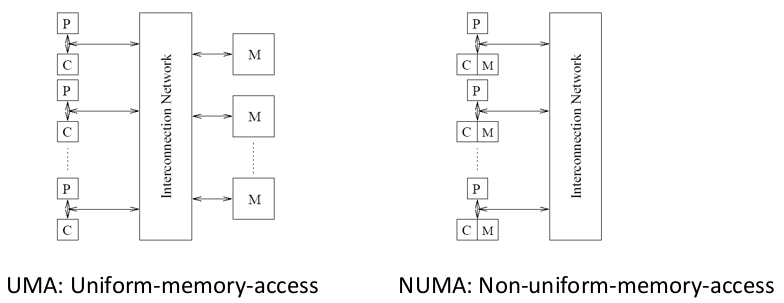
\includegraphics[width=0.8\textwidth]{figures/shared-address-space-platforms.png}
\caption{Shared Address Space Platforms}
\end{figure}

\hypertarget{uma}{%
\subsubsection{UMA}\label{uma}}

Uniform-memory-access shared-address-space computer with local caches
and global memories --\textgreater{} all memory access times (except
cache) are identical

\textit{E.g. Intel Pentium Front-Side Bus Evolution}

\hypertarget{numa}{%
\subsubsection{NUMA}\label{numa}}

Non-uniform-memory-access shared-address-space computer with local
memory only --\textgreater{} local memory access times are shorter.

\textit{E.g. Intel Core i7}

\hypertarget{cache-coherence}{%
\subsection{Cache coherence}\label{cache-coherence}}

\begin{itemize}
\tightlist
\item
  Cache

  \begin{itemize}
  \tightlist
  \item
    principle of space and time locality
  \item
    faster memory access
  \item
    additional hardware is required to keep multiple copies of data
    consistent with each other
  \end{itemize}
\item
  Cache Coherence

  \begin{itemize}
  \tightlist
  \item
    ensuring that concurrent operations on multiple copies of the same
    memory word have well-defined semantics
  \item
    this semantic is generally one of serializability
  \end{itemize}
\end{itemize}

\clearpage
\hypertarget{update-and-invalidate-protocols}{%
\subsubsection{Update and Invalidate
Protocols}\label{update-and-invalidate-protocols}}

When a processor changes the value of its copy of a variable, one of two
things must happen:

\begin{itemize}
\tightlist
\item
  the other copies must be invalidated (invalidate protocol)
  \textbf{(write-back)}
\item
  the other copies must be updated (update protocol)
  \textbf{(write-through)}
\end{itemize}

\hypertarget{pros-and-cons}{%
\paragraph{Pros and Cons}\label{pros-and-cons}}

\begin{itemize}
\tightlist
\item
  if a processor just reads a value once and does not need it again, an
  update protocol may generate significant overhead
\item
  if two processors make interleaved test and updates to a variable, an
  update protocol is better
\item
  both protocols suffer from false sharing overheads (two words that are
  not shared, however, they lie on the same cache line)
\end{itemize}

\hypertarget{today}{%
\paragraph{Today}\label{today}}

Most current machines use invalidate protocols

\begin{itemize}
\tightlist
\item
  each copy of a data item is associated with a state (e.g.~shared,
  invalid, or dirty)
\item
  in shared state, there are multiple valid copies of the data item
  (therefore, an invalidate would have to be generated on an update)
\item
  in dirty state, only one copy exists and therefore, no invalidates
  need to be generated
\item
  in invalid state, the data copy is invalid, therefore, a read
  generates a data request (and associated state changes)
\end{itemize}

\begin{figure}[H]
\centering
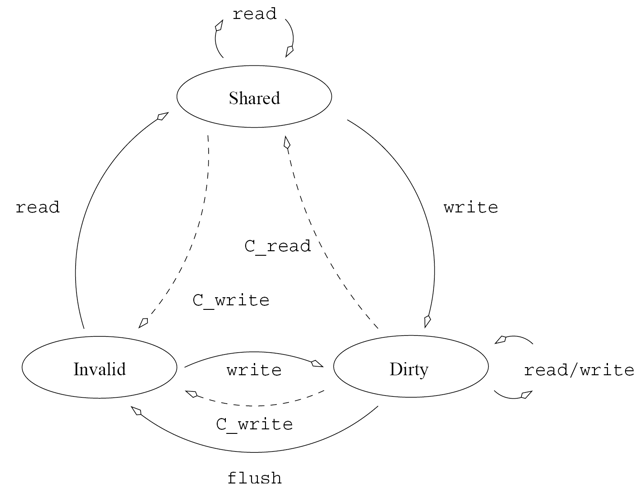
\includegraphics[width=0.7\textwidth]{figures/states-invalidate-protocols.png}
\caption{State Diagram of an invalidate protocol}
\end{figure}

\hypertarget{parallel-programming-in-c11}{%
\subsection{Parallel programming in
C++11}\label{parallel-programming-in-c11}}

\begin{itemize}
\tightlist
\item
  Explicit Threading

  \begin{itemize}
  \tightlist
  \item
    data exchange is more apparent

    \begin{itemize}
    \tightlist
    \item
      this helps in alleviating some of the overheads from data
      movement, false sharing, and contention
    \end{itemize}
  \item
    provides a richer API in the form of condition waits, locks of
    different types, and -increased flexibility for building composite
    synchronization operations
  \item
    tools and support are easier to find
  \end{itemize}
\item
  Directives Layered on Top of Threads

  \begin{itemize}
  \tightlist
  \item
    simplify a variety of thread-related tasks
  \item
    a programmer is rid of the tasks of initializing attributes objects,
    setting up arguments to threads, partitioning iteration spaces, etc.
  \end{itemize}
\end{itemize}

\hypertarget{threads-futures-tasks}{%
\subsection{Threads, Futures, Tasks}\label{threads-futures-tasks}}

\hypertarget{thread}{%
\subsubsection{Thread}\label{thread}}

\begin{itemize}
\tightlist
\item
  A thread is a single stream of control in the flow of a program.
\item
  low-level
\item
  exchange of data must be synchronized itself
\item
  uncaught exceptions in the thread function lead to the termination of
  the entire program
\item
  thread\_local storage class: static/global variables are created for
  each thread
\item
  is started automatically in the constructor
\item
  Constructor and Executor

  \begin{itemize}
  \tightlist
  \item
    thread( executable object, parameters of the executable object)
  \item
    Executable object

    \begin{itemize}
    \tightlist
    \item
      function object (functor)
    \item
      lambda expression
    \item
      pointer to a function
    \end{itemize}
  \item
    the executable object and the parameters are copied by default, so
    the thread can work on their own data
  \end{itemize}
\end{itemize}

\begin{lstlisting}[language=C++]
//FROM
void printFibs(size_t from, size_t to);

struct Image {
    void fill(int r, int g, int b);
};

//TO
int main() {
    thread th1(printFibs, 28, 35);
    Image img;
    thread th2([&img] { img.fill(0,1,2; });
    th1.join(); th2.join();
}
\end{lstlisting}

\hypertarget{future}{%
\subsubsection{Future}\label{future}}

\begin{itemize}
\tightlist
\item
  asynchronous processing: parallel execution or when calling get()

  \begin{itemize}
  \tightlist
  \item
    parallel or deferred processing
  \item
    async() initiates a computation and returns immediately
  \item
    get() blocks until the result of the computation is available
  \end{itemize}
\item
  exceptions appear in the parent thread when the result is picked up
  with get()
\item
  when leaving the scope of the responsible future, then its destructor
  ensures a clear and problem-free termination of the asynchronous
  computation
\item
  Return Value of async()

  \begin{itemize}
  \tightlist
  \item
    future, where RT is the return type of the asynchronously executed
    function
  \end{itemize}
\item
  Launch Policy

  \begin{itemize}
  \tightlist
  \item
    async(launch::async, longComputation) guarantees parallel execution
    (default)
  \item
    async(launch::deferred, computation) executed when calling get()
  \end{itemize}
\item
  a future can be produced without calling async(), by first creating a
  promise (some kind of transmission channel)
\end{itemize}

\begin{lstlisting}[language=C++]
#include <future>

static size_t fibrec(size_t n) {
    return (n < 2) ? 1 : fibrec(n - 2) + fibrec(n - 1);
}

int main() {
    // asynchronous computation
    auto fut1 = async(launch::async, &fibrec, 35);  // deferred computation
    auto fut2 = async(launch::deferred, &fibrec, 35);
    cout << fut2.get() << endl;        // waiting for the result of fut2
    cout << fut1.get() << endl;        // waiting for the result of fut1
}
\end{lstlisting}

\hypertarget{packaged-tasks}{%
\subsubsection{Packaged Tasks}\label{packaged-tasks}}

\begin{itemize}
\tightlist
\item
  Concept

  \begin{itemize}
  \tightlist
  \item
    a packaged\_task wraps a callable element and allows its result to
    be retrieved asynchronously
  \item
    it is similar to function, but transferring its result automatically
    to a future object
  \end{itemize}
\item
  Syntax

  \begin{itemize}
  \tightlist
  \item
    template \textless{}class Ret, class\ldots{} Args\textgreater{}
    class packaged\_task\textless{}Ret(Args\ldots{})\textgreater{};
  \end{itemize}
\item
  Object contains internally two elements

  \begin{itemize}
  \tightlist
  \item
    a stored task, which is some callable object whose call signature
    shall take arguments of the types in Args\ldots{} and return a value
    of type Ret
  \item
    a shared state, which is able to store the results of calling the
    stored task (of type Ret) and be accessed asynchronously through a
    future
  \end{itemize}
\end{itemize}

\begin{lstlisting}[language=C++]
// create task for calling fibrec
// argument of fibrec has to be defined later
packaged_task<size_t(size_t)> task1(&fibrec);
auto f1 = task1.get_future(); // future for getting result
// create task for calling fibrec
// argument of fibrec is bound to 35
packaged_task<size_t(void)> task2(bind(&fibrec, 35));
auto f2 = task2.get_future(); // future for getting result
// call task1 in a parallel thread (move semantic)
thread th(move(task1), 35);
// call task2 in this tread
task2();
// get results
cout << f1.get() << endl;
cout << f2.get() << endl;
th.join(); // this treads waits on parallel thread th
\end{lstlisting}

\hypertarget{synchronization-primitives}{%
\subsubsection{Synchronization
Primitives}\label{synchronization-primitives}}

\begin{itemize}
\tightlist
\item
  Synchronized data access (read and write) is necessary if at least one
  of the parallel threads changes common data
\item
  Synchronization Primitives
\end{itemize}

\begin{figure}[H]
\centering
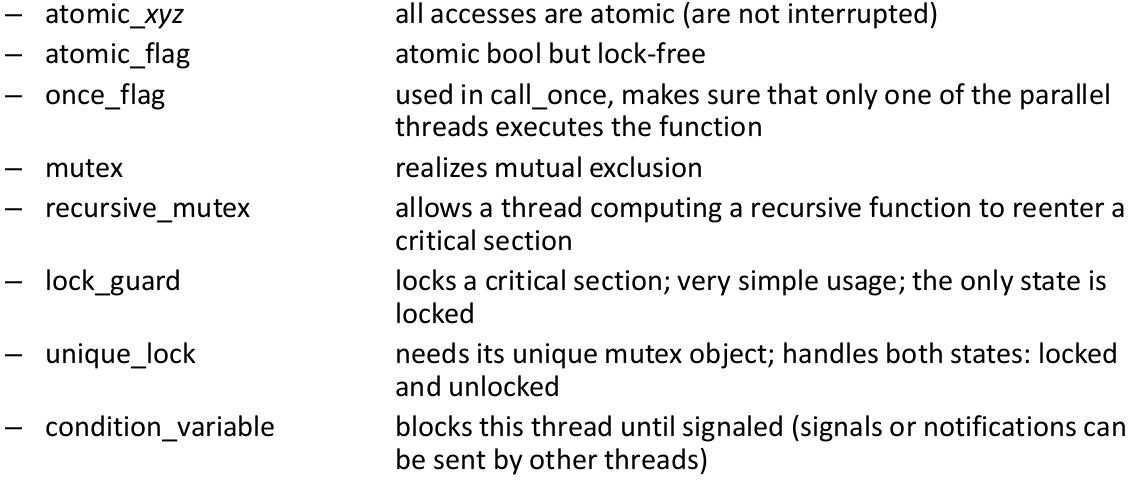
\includegraphics[width=0.7\textwidth]{figures/sync-primitives.png}
\caption{Synchronization Primitives}
\end{figure}

\hypertarget{serial-for--vs.parallel-for-loop}{%
\subsubsection{Serial for- vs.~Parallel
for-Loop}\label{serial-for--vs.parallel-for-loop}}

\begin{itemize}
\tightlist
\item
  Notice

  \begin{itemize}
  \tightlist
  \item
    a lot of programming languages don't have a special parallel
    for-loop syntax
  \item
    they use the keyword for in two situations
  \end{itemize}
\item
  Serial for-Loop

  \begin{itemize}
  \tightlist
  \item
    the loop notation simplifies the programming of a fixed number of
    repetitive, sequentially ordered steps

    \begin{itemize}
    \tightlist
    \item
      \textit{Example: reading n integers from a sequential file}
    \end{itemize}
  \end{itemize}
\item
  Parallel for-Loop

  \begin{itemize}
  \tightlist
  \item
    the loop notation simplifies the programming of a fixed number of
    repetitive steps, that can be done in any order

    \begin{itemize}
    \tightlist
    \item
      \textit{Example: for each element of an array proceed the same task}
    \end{itemize}
  \end{itemize}
\end{itemize}

The C++ platforms provide proprietary parallel algorithms and data
structures, but not in standard.

\hypertarget{parallel-for-each-implementation}{%
\subsubsection{Parallel for-each
Implementation}\label{parallel-for-each-implementation}}

\begin{lstlisting}[language=C++]
//Just an example of how an implementation for a parallel for-each loop could look like.

template<typename It>
void parallelForEach(It first, It last, function<void(typename It::reference)> f) {
    const ptrdiff_t len = last - first;
    if (len == 0) {
        return;
    } else if (len == 1) {
        f(*first);
        return;
    }

    const It mid = first + (ptrdiff_t)(len/2);
    future<void> bgTask = async(parallelForEach<It>, first, mid, f);
    try {
        parallelForEach(mid, last, f);
    } catch (...) {
        bgTask.wait();
        throw;
    }
    bgTask.get();
}
\end{lstlisting}

\clearpage
\hypertarget{visual-c-concurrency-runtime}{%
\subsection{Visual C++ concurrency
runtime}\label{visual-c-concurrency-runtime}}

The concurrency runtime provides uniformity and predictability to
applications that run simultaneously

Benefits are:

\begin{itemize}
\tightlist
\item
  cooperative task scheduling (work-stealing algorithm)
\item
  cooperative blocking (the remaining quantum can be used to perform
  another task as the first task waits for the resource)
\end{itemize}

\begin{figure}[H]
\centering
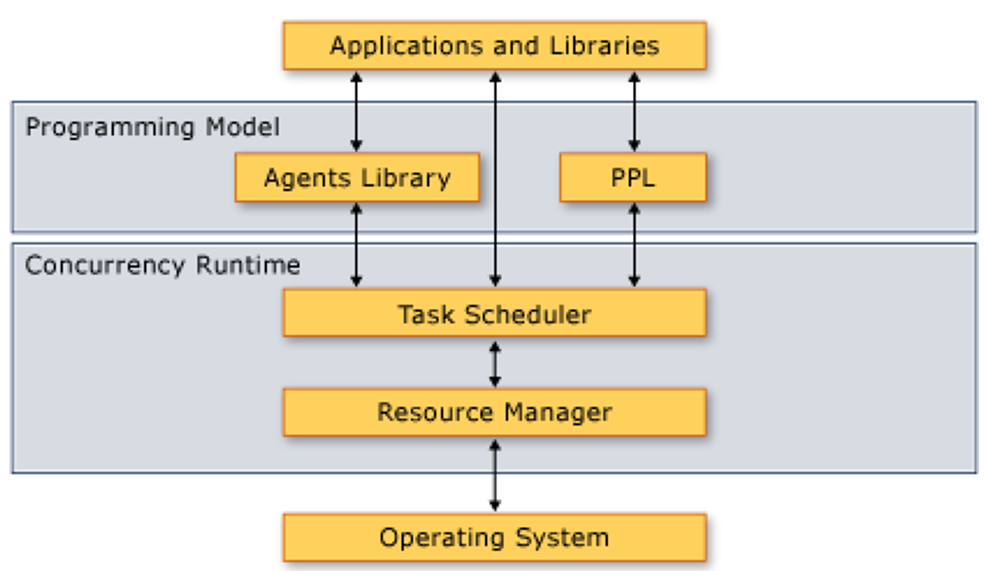
\includegraphics[width=0.7\textwidth]{figures/parallel-architecture.png}
\caption{Concurrency Runtime Architecture}
\end{figure}

\begin{itemize}
\tightlist
\item
  Parallel Patterns Library (PPL)

  \begin{itemize}
  \tightlist
  \item
    provides general-purpose containers and algorithms for performing
    fine-grained parallelism
  \end{itemize}
\item
  Asynchronous Agents Library

  \begin{itemize}
  \tightlist
  \item
    actor-based programming model
  \item
    message passing interface for coarse-grained dataflow
  \end{itemize}
\end{itemize}

\hypertarget{concurrency-runtime-vs.openmp}{%
\subsubsection{Concurrency Runtime
vs.~OpenMP}\label{concurrency-runtime-vs.openmp}}

\begin{itemize}
\tightlist
\item
  OpenMP

  \begin{itemize}
  \tightlist
  \item
    well-suited for parallel algorithms that are iterative
  \item
    is most efficient when the degree of parallelism is pre-determined
    and matches the available resources on the system
  \item
    the OpenMP model is an especially good match for high-performance
    computing

    \begin{itemize}
    \tightlist
    \item
      where very large computational problems are distributed across the
      processing resources of a single computer
    \item
      the hardware environment is known
    \item
      the developer can reasonably expect to have exclusive access to
      computing resources when the algorithm is executed
    \end{itemize}
  \end{itemize}
\item
  Concurrency Runtime

  \begin{itemize}
  \tightlist
  \item
    useful in less constrained computing environments
  \item
    recursive problems (such as the quicksort algorithm or searching a
    tree of data) are
  \item
    easier to implement by using the Concurrency Runtime
  \item
    provides a dynamic scheduler that adapts to available resources and
    adjusts the degree of parallelism as workloads change
  \item
    many of the features can be extended or composed to new ones
  \end{itemize}
\end{itemize}

\hypertarget{new-features-in-c17}{%
\subsubsection{New Features in C++17}\label{new-features-in-c17}}

\begin{itemize}
\tightlist
\item
  Ordering (since C++11)

  \begin{itemize}
  \tightlist
  \item
    ``sequenced-before'' is an asymmetric, transitive, pair-wise
    relationship between evaluations within the same thread
  \item
    if A is sequenced before B, then evaluation of A will be complete
    before evaluation of B begins
  \item
    if A is not sequenced before B and B is not sequenced before A, then
    two possibilities exist:

    \begin{itemize}
    \tightlist
    \item
      evaluations of A and B are indeterminately sequenced: they may be
      performed in any order but may not overlap: either A will be
      complete before B, or B will be complete before A
    \item
      evaluations of A and B are unsequenced: they may be performed in
      any order and may overlap (within a single thread of execution,
      the compiler may interleave the CPU instructions that comprise A
      and B)
    \end{itemize}
  \end{itemize}
\item
  Execution Policies in C++17

  \begin{itemize}
  \tightlist
  \item
    most algorithms have overloads that accept execution policies:

    \begin{itemize}
    \tightlist
    \item
      std::execution::seq\\
      sequential execution
    \item
      std::execution::par\\
      parallel execution is allowed parallel instructions are
      indeterminately sequenced
    \item
      std::execution::par\_unseq\\
      execution may be parallelized, vectorized, or migrated across
      threads\\
      parallel instructions and ordering in the same thread: unsequenced
    \end{itemize}
  \end{itemize}
\end{itemize}

\begin{lstlisting}[language=C++]
int a[] = { 0, 1 };
vector<int> v;
for_each(execution::par, begin(a), end(a), [&](int i) {
    v.push_back(i*2+1); // Error: data race (vector isn't thread safe)
});

int x = 0;
mutex m;
for_each(execution::par, begin(a), end(a), [&](int) {
    lock_guard<mutex> guard(m);
    ++x;     // Correct, because mutual exclusion is guaranteed
});    // and sequential is irrelevant
\end{lstlisting}

\hypertarget{openmp}{%
\subsection{OpenMP}\label{openmp}}

A standard for directive based parallel programming

\begin{itemize}
\tightlist
\item
  OpenMP is a directive-based API that can be used with

  \begin{itemize}
  \tightlist
  \item
    FORTRAN
  \item
    C/C++
  \item
    for programming shared address space machines
  \end{itemize}
\item
  OpenMP directives provide support for

  \begin{itemize}
  \tightlist
  \item
    concurrency
  \item
    synchronization
  \item
    data handling
  \end{itemize}
\item
  OpenMP in C/C++

  \begin{itemize}
  \tightlist
  \item
    directives are based on the \#pragma compiler directives
  \item
    a directive consists of a directive name followed by clauses
  \item
    \#pragma omp directive {[}clause list{]}
  \end{itemize}
\item
  OpenMP programs

  \begin{itemize}
  \tightlist
  \item
    execute serially until they encounter the parallel directive, which
    creates a group of threads\\
    \#pragma omp parallel {[}clause list{]}\\
    /* structured block */
  \item
    the main thread that encounters the parallel directive becomes the
    master of this group of threads and is assigned the thread id 0
    within the group
  \item
    at the end of the parallel executed block the main thread waits for
    all parallel threads (join)
  \end{itemize}
\end{itemize}

\hypertarget{clause-list-in-openmp}{%
\subsubsection{Clause List in OpenMP}\label{clause-list-in-openmp}}

\begin{itemize}
\tightlist
\item
  Clause List specifies

  \begin{itemize}
  \tightlist
  \item
    Conditional Parallelization

    \begin{itemize}
    \tightlist
    \item
      the clause if (scalar expr) determines whether the parallel
      construct results in creation of threads
    \item
      the scalar expression is evaluated at runtime
    \end{itemize}
  \item
    Degree of Concurrency

    \begin{itemize}
    \tightlist
    \item
      the clause num\_threads(integer expr) specifies the number of
      threads that are created
    \end{itemize}
  \item
    Data Handling

    \begin{itemize}
    \tightlist
    \item
      the clause private (variable list) indicates variables local to
      each thread T
    \item
      the clause firstprivate (variable list) is similar to the private,
      except values of variables are initialized to corresponding values
      before the parallel directive
    \item
      the clause shared (variable list) indicates that variables are
      shared across all the threads
    \end{itemize}
  \end{itemize}
\end{itemize}

\begin{lstlisting}[language=C++]
#pragma omp parallel if(is_parallel == 1) num_threads(8) \
private(a) shared(b) firstprivate(c)
{
    /* structured block */
}
\end{lstlisting}

\hypertarget{default-clause-in-openmp}{%
\subsubsection{Default Clause in
OpenMP}\label{default-clause-in-openmp}}

\begin{itemize}
\tightlist
\item
  Syntax

  \begin{itemize}
  \tightlist
  \item
    default(shared \textbar{} none)
  \end{itemize}
\item
  Semantic

  \begin{itemize}
  \tightlist
  \item
    the default clause allows the user to affect the data-sharing
    attributes of variables
  \item
    omitting this clause is the same as default(shared)
  \end{itemize}
\item
  default(shared)

  \begin{itemize}
  \tightlist
  \item
    is equivalent to explicitly listing each currently visible variable
    in a shared clause, unless it is threadprivate or const-qualified
  \end{itemize}
\item
  default(none)

  \begin{itemize}
  \tightlist
  \item
    it is usually better style to use default(none) instead of
    default(shared)
  \item
    requires that at least one of the following must be true for every
    reference to a variable in the lexical extent of the parallel
    construct
  \end{itemize}
\end{itemize}

\clearpage
\hypertarget{reduction-clause-in-openmp-important}{%
\subsubsection{Reduction Clause in OpenMP
(important)}\label{reduction-clause-in-openmp-important}}

\begin{itemize}
\tightlist
\item
  specifies how multiple local copies of a variable at different threads
  are combined into a single copy at the master when threads exit
\item
  the usage is reduction (operator: variable list)
\item
  the variables in the list are implicitly specified as being private to
  threads
\item
  the operator can be one of +, *, -, \&, \textbar{}, \^{}, \&\&, and
  \textbar{}\textbar{}
\end{itemize}

\begin{lstlisting}[language=C++]
#pragma omp parallel default(none) reduction(+: sum) num_threads(8)
{
    /* compute local sums here */
    sum = ...;
}
/*sum here contains sum of all local instances of sums */
\end{lstlisting}

\hypertarget{concurrent-tasks-in-openmp}{%
\subsection{Concurrent tasks in
OpenMP}\label{concurrent-tasks-in-openmp}}

\hypertarget{the-for-directive}{%
\subsubsection{The for Directive}\label{the-for-directive}}

\begin{itemize}
\tightlist
\item
  specifies concurrent iterations
\item
  is used to split parallel iteration spaces across threads
\item
  the general form is\\
  \#pragma omp for {[}clause list{]}
\end{itemize}

\hypertarget{schedule-clause}{%
\paragraph{Schedule Clause}\label{schedule-clause}}

\begin{itemize}
\tightlist
\item
  Schedule Clause

  \begin{itemize}
  \tightlist
  \item
    deals with the assignment of iterations to threads
  \item
    the general form of the schedule directive is
    schedule(scheduling\_class{[}, parameter{]})
  \end{itemize}
\item
  four scheduling classes

  \begin{itemize}
  \tightlist
  \item
    static

    \begin{itemize}
    \tightlist
    \item
      splits the iteration space into equal chunks of size parameter and
      assigns them to threads in a round-robin fashion
    \item
      when no parameter is specified, the iteration space is split into
      equally sized chunks, one chunk per thread
    \end{itemize}
  \item
    dynamic

    \begin{itemize}
    \tightlist
    \item
      the iteration space is partitioned into chunks of size parameter
      (default value: 1)
    \item
      these chunks are assigned to threads as they become idle
    \end{itemize}
    \clearpage
  \item
    guided

    \begin{itemize}
    \tightlist
    \item
      the chunk size is reduced exponentially as each chunk is
      dispatched to a thread
    \item
      the parameter specifies the smallest chunk size (default value: 1)
    \end{itemize}
  \item
    runtime

    \begin{itemize}
    \tightlist
    \item
      the environment variable OMP\_SCHEDULE determines at runtime the
      scheduling class and the chunk size
    \end{itemize}
  \end{itemize}
\end{itemize}

\hypertarget{the-nowait-clause}{%
\paragraph{The nowait Clause}\label{the-nowait-clause}}

\begin{itemize}
\tightlist
\item
  Implicit Barrier

  \begin{itemize}
  \tightlist
  \item
    at the end of the parallel for-loop all threads join
  \end{itemize}
\item
  Clause nowait

  \begin{itemize}
  \item
    often, it is desirable to have a sequence of for-directives within a
    parallel construct that do not execute an implicit barrier at the
    end of each for directive

\begin{lstlisting}[language=C++]
#pragma omp parallel
{
    #pragma omp for nowait
    for (int i = 0; i < nmax; i++)
        if (isEqual(name, current_list[i]) processCurrName(name);
    #pragma omp for
    for (int i = 0; i < mmax; i++)
        if (isEqual(name, past_list[i]) processPastName(name);
}
\end{lstlisting}
  \end{itemize}
\end{itemize}

\hypertarget{the-sections-directive}{%
\subsubsection{The sections Directive}\label{the-sections-directive}}

\begin{itemize}
\item
  specifies concurrent tasks
\item
  supports non-iterative parallel task assignment using the sections
  directive
  
 \begin{lstlisting}[language=C++]
#pragma omp sections [clause list]
{
    #pragma omp section
    {
        taskA();
    }
    #pragma omp section
    {
        taskB();
    }
    ...
}
 \end{lstlisting}
\end{itemize}

\clearpage
\hypertarget{merging-directives}{%
\subsubsection{Merging Directives}\label{merging-directives}}

\begin{itemize}
\tightlist
\item
  Remember

  \begin{itemize}
  \tightlist
  \item
    the parallel directive creates the group of threads
  \item
    the for and the sections directive would execute serially (by the
    master thread) if no parallel directive is specified before
  \end{itemize}
\item
  You are able to merge directives like ``\#pragma omp parallel
  shared(n)'' and ``\#pragma omp for'' to ``\#pragma omp parallel for
  shared(n)''
\end{itemize}

\hypertarget{nesting-parallel-directives}{%
\subsubsection{Nesting parallel
Directives}\label{nesting-parallel-directives}}

\begin{itemize}
\tightlist
\item
  OpenMP does not allow nested for, sections, and single directives that
  bind to the same parallel directive
\item
  each for directive brings its own parallel directive, which only
  generates a logical team of threads on encountering a nested parallel
  directive
\item
  the newly generated logical team is still executed by the same thread
  corresponding to the outer parallel directive
\item
  to generate a new set of threads, nested parallelism must be enabled
  by setting the OMP\_NESTED environment variable to TRUE
\end{itemize}

\hypertarget{synchronization-in-openmp}{%
\subsection{Synchronization in OpenMP}\label{synchronization-in-openmp}}

\begin{itemize}
\tightlist
\item
  \#pragma omp barrier
\item
  \#pragma omp single {[}clause list{]} structured block
\item
  \#pragma omp master structured block
\item
  \#pragma omp critical {[}(name){]} structured block
\item
  \#pragma omp atomic memory update instruction
\item
  \#pragma omp ordered structured block
\item
  \#pragma omp flush {[}(variable list){]}
\end{itemize}

\hypertarget{example-prefix-sums}{%
\subsubsection{Example: Prefix Sums}\label{example-prefix-sums}}

 \begin{lstlisting}[language=C++]
cumulSum[0] = list[0];
#pragma omp parallel for default(none) shared(cumulSum, list) ordered
for (int i = 1; i < n; i++) {
    // other work
    #pragma omp ordered
    {
        cumulSum[i] = cumulSum[i - 1] + list[i];
    }
}
\end{lstlisting}

\hypertarget{openmp-library-functions}{%
\subsection{OpenMP library functions}\label{openmp-library-functions}}

\begin{figure}[H]
\centering
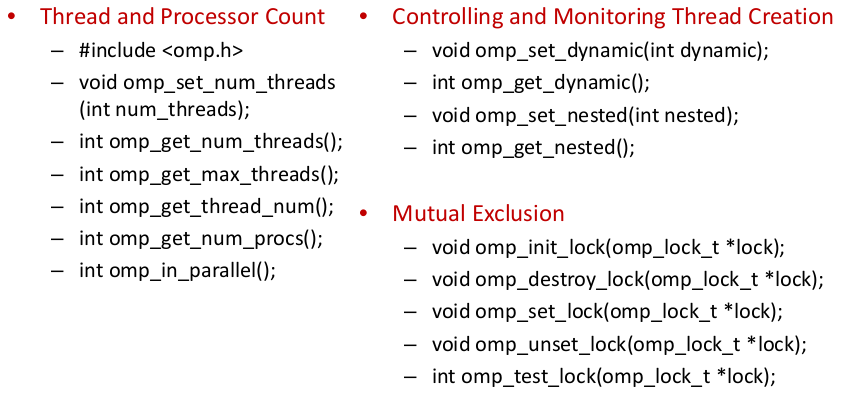
\includegraphics[width=0.7\textwidth]{figures/openMp-Library-Function.png}
\caption{OpenMP Library Functions}
\end{figure}

\begin{itemize}
\tightlist
\item
  OMP\_NUM\_THREADS
\item
  OMP\_SET\_DYNAMIC
\item
  OMP\_NESTED
\item
  OMP\_SCHEDULE
\end{itemize}

\clearpage